% intro
Performing voxel-based (or "backwards") reconstruction is not as straight forward as the pixel-based method. For each voxel, one must find the b-scan that is closest when transformed into the volume. When found, the pixel on this b-scan that will contribute to the voxel must then be located. In this section, the voxel-based reconstruction implemented in this thesis is described. As in the previous section on pixel-based reconstruction, we also cover how this is parallelized on the GPU and some of the important optimization techniques.

% description of the steps
\subsection{Method}

%	(interpolate and calibrate)
%	fill plane_points
%	transform plane_points
%	fill b-scan_plane_equations from plane_points
%	for each voxel:
	%	calculate distance to planes, find smallest distance
	%	use plane normal and distance to get projected point
	%	subtract corner0 and project on x- and y-vector to get 2D coordinates
	%	divide by b-scan spacing to convert to pixel indices
	%	fill voxel with pixel intensity using compounding methods
	
The method is based on voxel-nearest-neighbor (VNN) \cite{sherebrin1996}. As with pixel-based reconstruction, the input tracking data must be calibrated and interpolated. After this has been completed, the two approaches start differ. The reconstruction consists of the following steps illustrated in Figure \ref{fig:non-inc_vnn}.

	\begin{figure}[h]
	\centering
	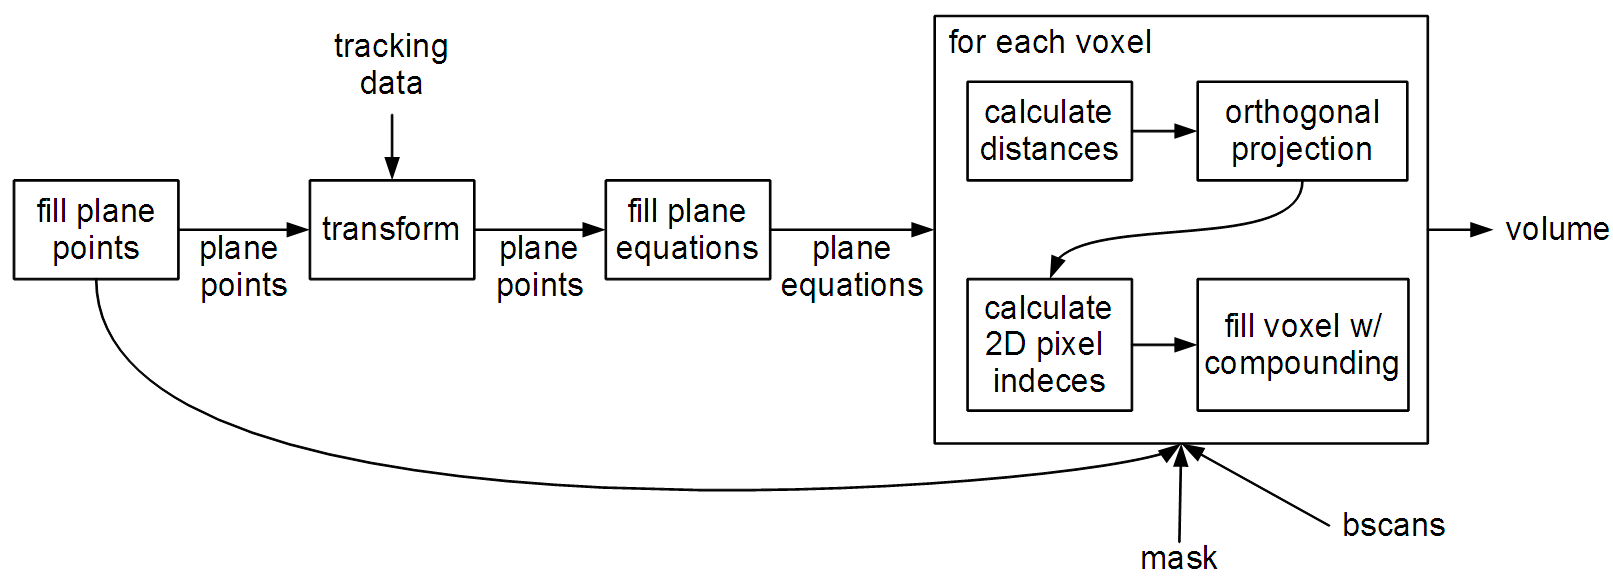
\includegraphics[width=\textwidth]{graphics/non-inc_vnn.png}
	\caption{Steps performed in voxel-based reconstruction}
	\label{fig:non-inc_vnn}
	\end{figure}

\begin{enumerate}
	\item Fill $planepoints$
	\item Transform $planepoints$
	\item Fill $planeequations$ from transformed $planepoints$
	\item For each voxel:
	\begin{enumerate}
		\item Calculate distance from voxel to planes
		\item Calculate orthogonal projection of voxel on closest plane
		\item Calculate 2D coordinates of projection on plane and convert to pixel indices
		\item Fill voxel using compounding methods
	\end{enumerate}
\end{enumerate}

In the first step an array of $n$ triplets of 3D space locations is constructed. The points in the triplet are the top-left, bottom-left and top-right corners of the b-scans in world coordinate space such that all b-scans are parallel and lie flat on the YZ plane. See Equation \ref{eq:plane_points}. The top-left corner is dubbed $corner0$, the top-right $cornerx$ and the bottom-left $cornery$.

\begin{equation}
\label{eq:plane_points}
	corner0 = (0,0,0), \; cornerx = (0,w\Delta x,0), \; cornery = (0,0,h\Delta y)
\end{equation}

In the second step, these points are transformed according to the tracking data. The transformation matrix of each b-scan is multiplied by each of the three corners, and the resulting coordinates are now correctly placed in world space. Three points is enough to define a plane, but to avoid redundant calculations, an array of $n$ plane equations is constructed in step three. Equations \ref{eq:pp2pe0} and \ref{eq:pp2pe1} show how three b-scan corners are used to calculate the parameters of a plane equation. Each plane equation has four parameters, $A$, $B$, $C$ and $D$, and define a plane implicitly. The plane equation is given in Equation \ref{eq:plane_equation}. The mathematically inclined reader will notice that A, B and C are vector coordinates of the plane normal, and D is the distance from origin to the closest point on the plane.

\begin{equation}
\label{eq:pp2pe0}
	normal = \frac{(corner0-cornerx) \times (cornery-corner0)}{|(corner0-cornerx) \times (cornery-corner0)|}
\end{equation}

\begin{equation}
\label{eq:pp2pe1}
	(A,B,C,D) = (normal_x, normal_y, normal_z, -A\cdot normal)
\end{equation}

\begin{equation}
\label{eq:plane_equation}
	Ax + By + Cz + D = 0
\end{equation}

The last step is to iterate over all voxels and fill their value from the closest b-scan. It is for this purpose that $planepoints$ and $planeequations$ were constructed in the previous steps. To fill a voxel, a series of \emph{substeps} are performed (see previous list). Each voxel with indices $(x,y,z)$ has world space coordinates given by $v = (x\Delta v,y\Delta v,z\Delta v)$. In the first substep (a), we calculate the distance of an orthogonal projection from these coordinates to each of the b-scan planes and find the minimum. The brute force approach is to test all planes, but a clever optimization technique has been devised and will be explained under "Optimization Techniques" below. For a point $v$, the orthogonal distance to a plane is found using Equation \ref{eq:distance}.

\begin{equation}
\label{eq:distance}
	distance = \frac{(A,B,C)\cdot v + D}{|(A,B,C)|}
\end{equation}

The next substep (b) is then to calculate the world space coordinates $p$ of the voxel coordinates orthogonally projected onto the plane. Given the distance and the plane normal, this is given as Equation \ref{eq:p}.

\begin{equation}
\label{eq:p}
	p = v - distance\cdot (A,B,C)
\end{equation}

To fill the voxel, we need the pixel intensity at this location ($p$) on the b-scan. This requires calculating the pixel indices in the b-scan image. To do this, substep (c), the vector from the top-left corner ($corner0$) to the point $p$ is projected onto normalized vectors parallel with the x and y axis of the b-scan. The lengths of the projections are divided by $\Delta x$ and $\Delta y$ to give pixel indices $(px,py)$. Equations \ref{eq:pxy0} and \ref{eq:pxy1} show the calculations.

\begin{equation}
\label{eq:pxy0}
	px = \frac{(p-corner0) \cdot |cornerx-corner0|}{\Delta x}
\end{equation}

\begin{equation}
\label{eq:pxy1}
	py = \frac{(p-corner0) \cdot |cornery-corner0|}{\Delta y}
\end{equation}

Given the indices of the contributing pixel, the last substep (d) is to fill the voxel with the calculated value.

% description of how data/work is split up for parallelization,
% and also what parts are done on the CPU and GPU
\subsection{Parallelization}

% All except voxel filling step done on CPU
% NDRange of volume_w x volume_n to utilize modified fast slice selection
% work group size of 512

A code listing of the implemented OpenCL kernel can be found in Appendix \ref{section:vnn_kernel}. In the previously described method, only step 4 is computationally demanding enough to require parallelization. There are only three points and one equation per input b-scan, and as there are typically around 200-500 such b-scans, the total computation time is negligible compared to iterating over all the voxels. For example, volume size can typically be $256^3$ or $512^3$. Also, the sizes of the corner points and equation parameters are small enough to be quickly transferred to the device. To summarize, step 1 to 3 is performed on the CPU, and step 4 is parallelized on the GPU.

The voxels are processed concurrently in columns. A volume of $w_{volume} \times h_{volume} \times n_{volume}$ voxels will result in $w_{volume} \times n_{volume}$ threads. Each thread executes a kernel that iterates over $h_{volume}$ voxels, performing substep (a) to (d) on each to fill them. The reason for this separation is that each voxel processed in a column is not more than than $\Delta v$ from the previously processed voxel, and this property is used in an optimization technique to be described below.

% description of various tricks and optimizations done
\subsection{Optimization Techniques}

%	NDRange optimizations
%	Modified fast slice selection!
	%	Process voxels in columns
	%	Search all planes for closest to first voxel in column
	%	for each voxel in column:
		%	"annenhver utover" from last closest plane
		%	break when difference between closest and current plane is above cutoff (it has peaked)
		
	During voxel-based reconstruction, one of the most computationally demanding tasks is to find the b-scan that is closest to a voxel. The brute force approach involves testing all $n$ b-scans for each of the $w_{volume} \times h_{volume} \times n_{volume}$ voxels, a computationally expensive task. However, it is possible to exploit inherent continuity in the b-scans.
	
	% Wein \textit{et al.}\ \cite{wein2006} describe a fast way to decide the closest b-scan, by iterating over the voxels in a pattern such that each processed voxel is next to the previously processed voxel. 
	
	Ideally, each b-scan will come "after" the previous one. In other words no b-scan will intersect another, and each b-scan is in front of the previous (in the direction of the probe's trajectory). Noise in the tracking data and an unsteady hand can cause the b-scans to be partially shuffled. Additionally, when rotating the probe, there is a high probability that b-scans will intersect each other. Even though the b-scans may come in any order, the general tendency is along the probe trajectory. In other words, they are \emph{partially ordered}. This means that if the closest b-scan to a given voxel is found, then the index of the closest b-scan to the neighbor voxel is probably close to the index of the previously closest b-scan. To take advantage of this, the following scheme was devised:
	
	\begin{itemize}
		\item Let each thread process a column of voxels
		\item $i$ = index of b-scan closest to first voxel in column found by brute force
		\item For each voxel in column:
		\begin{itemize}
			\item Loop $j \in {0, 1, 2, ..., n}$
			\begin{itemize}
				\item Calculate distance to b-scans with index $k=i+j$ and $l=i-j$ (if they exist)
				\item $i$ = the closest b-scan of $i$, $k$ and $l$
				\item If difference between distance to $i$ and distance to $k$ or $l$ is above a given cutoff, stop testing any more $k$s or $l$s, respectively
			\end{itemize}
		\end{itemize}
	\end{itemize}
	
	The idea is that b-scans before and after the previous b-scan that was closest are tested. It is important to process voxels next to each other and not, for instance, jump from voxel $(w-1,y,z)$ to $(0,y+1,z)$ because they are neighbors in memory. Since the b-scans are partially ordered the assumption is that when testing a  b-scan with an index far enough from the last b-scan that was closest, it will not be a better (closer) choice than the b-scans tested so far. The cutoff limit will depend on the nature of the input tracking data. For example, in one of our test cases, a cutoff of $4\Delta v$ was sufficient. After this, the distances found had "peaked", and the search could end.